\documentclass{standalone}
\usepackage{tikz}

\usetikzlibrary{calc,shadows}


\begin{document}

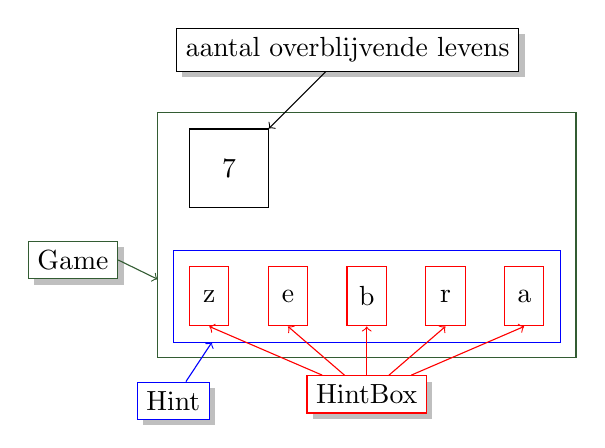
\begin{tikzpicture}[hintbox/.style={draw=red,minimum width=0.5cm,minimum height=0.75cm},
                    note/.style={drop shadow,fill=white,draw}]
  \foreach[count=\i] \c in {z,e,b,r,a} {
    \node[hintbox,anchor=south west] (hintbox \c) at (\i,0) {\c};
  }

  \node[minimum width=1cm,minimum height=1cm,draw,anchor=south west] (lives) at (1,1.5) {7};

  \coordinate (hint south west) at ($ (hintbox z.south west) + (-.2,-.2) $);
  \coordinate (hint north east) at ($ (hintbox a.north east) + (.2,.2) $);
  \coordinate (hint south east) at (hint south west -| hint north east);
  \coordinate (hint north west) at (hint south west |- hint north east);

  \draw[draw=blue] (hint south west) rectangle (hint north east);

  \coordinate (game south west) at ($ (hintbox z.south west) + (-.4,-.4) $);

  \path let \p1=(lives.north east), \p2=(hintbox a.north east) in
        [draw=green!20!black!80] (game south west) rectangle ($ (\x2, \y1) + (.4,.2) $);

  \node[note] (note lives) at ($ (lives.north east) + (1,1) $) { aantal overblijvende levens };
  \draw[->] (note lives) -- (lives);

  \node[note,anchor=north,draw=blue] (note hint) at ($ (hint south west) + (0,-.5) $) {Hint};
  \draw[->,blue] (note hint) -- ($ (hint south west) ! 0.1 ! (hint south east) $);

  \node[note,anchor=north,draw=red] (note hintbox) at ($ (hintbox b) + (0,-1) $) {HintBox};
  \foreach \c in {z,e,b,r,a} {
    \draw[->,red] (note hintbox) -- ($ (hintbox \c.south) $);
  }

  \node[note,draw=green!20!black!80,anchor=south east] (note game) at ($ (game south west) + (-.5,1) $) {Game};
  \draw[->,green!20!black!80] (note game.east) -- ($ (game south west) + (0,1) $);
\end{tikzpicture}



\end{document}